\section{Preliminaries}
\subsection{Proofs using the Curry-Howard Correspondence}
The Curry-Howard correspondence is a way to interpret typed computer programs as mathematical proofs \cite{chc}. This is done by representing false statements as empty types, and true statements as non-empty types. For example, take  \verb|IsTrue b|  where  \verb|b| is some boolean. The type is constructed in such a way that it is empty if  \verb|b| is false, and non-empty if b is true.  If one has a value of type  \verb|IsTrue b|, this value (often called a witness) is a proof that  \verb|b| must be true. 

These proofs can be used as function arguments, constructor arguments or even as a function result. Since Agda is dependently typed, the proof can also refer to other arguments of a function. For example, this function may only be called when \verb|n| is greater than 3:
\begin{minted}{agda}
takesGtFive : (n : Nat) -> IsTrue (n > 5) -> ?
\end{minted}

\subsection{QuadTrees}
The QuadTree is a data structure that is used for storing two-dimensional information in a functional way \cite{Finkel1974}. It is defined as:
\begin{minted}{haskell}
data Quadrant t = Leaf t
        | Node (Quadrant t) (Quadrant t) (Quadrant t) (Quadrant t)

data QuadTree t = Wrapper (Nat, Nat) (Quadrant t)
\end{minted}

\begin{wrapfigure}{r}{0.3\textwidth} %this figure will be at the right
    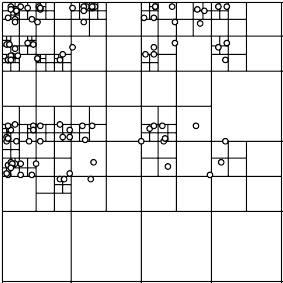
\includegraphics[width=0.3\textwidth]{graphics/test.png}
    \caption{An example QuadTree}
    \label{quadtree}
\end{wrapfigure}

A QuadTree consists of the size (width  ×  height) of the QuadTree, and the root quadrant. A quadrant is either a leaf (in which case all the values inside the region of the quadrant are the same), or four subquadrants. The four subquadrants are then called A (top left), B (top right), C (bottom left), and D (bottom right). Notice that in Figure \ref{quadtree}, space is consistently split into four quadrants.

There are five functions that can be used to interact with QuadTrees:
\begin{minted}{haskell}
-- Create a new QuadTree with the specified size
makeTree :: (Nat, Nat) -> t -> QuadTree t
-- Get a lens to the specified location
atLocation :: (Nat, Nat) -> Lens (QuadTree t) t
-- Get the value at the specified location
getLocation :: (Nat, Nat) -> QuadTree t -> t
-- Set the value at the specified location
setLocation :: (Nat, Nat) -> t -> QuadTree t -> QuadTree t
-- Map the value at the specified location
mapLocation :: (Nat, Nat) -> (t -> t) -> QuadTree t -> QuadTree t
\end{minted}

\subsection{Lenses}
The QuadTree library makes extensive use of Lenses. Lenses are composable functional references \cite{lens}. They allow one to access and modify data in some data structure. This paper chooses to use the Van Laarhoven representation \cite{laarhovenlens}, since this is what the original library used. It is defined as:
\begin{minted}{haskell}
type Lens s a = forall f. Functor f => (a -> f a) -> s -> f s
\end{minted}
Using this representation, \verb|Lens a b| means that given an object of type \verb|a|, we can view or modify an inner object of type \verb|b|.
The functions to interact with Lenses are:
\begin{minted}{haskell}
-- Get the value at this lens
view :: Lens a b -> a -> b
-- Set the value at this lens
set :: Lens a b -> b -> a -> a
-- Map the value at this lens
over :: Lens a b -> (b -> b) -> a -> a
-- Compose two lenses (Note: This is actually just regular function composition!)
compose :: Lens a b -> Lens b c -> Lens a c
\end{minted}